\documentclass[oneside,a4paper,14pt]{extarticle}
\usepackage[T1,T2A]{fontenc}
\usepackage[
a4paper,
top=2cm,
bottom=2cm,
left=2.5cm,
right=1.5cm
]{geometry}
\usepackage[utf8]{inputenc}
\usepackage[russian]{babel}
\usepackage{textcomp}
\usepackage{indentfirst}
\usepackage{listings}
\usepackage{listingsutf8}
\usepackage{xcolor}
\usepackage{float}
\usepackage{enumitem}
\usepackage{graphicx}
\usepackage{mwe}
\usepackage{wrapfig}
\usepackage{caption}
\usepackage{amsmath}
\usepackage{amsfonts}
\usepackage{amsthm}
\usepackage[all]{xy}
\usepackage[breaklinks]{hyperref}
\usepackage{xurl}
\usepackage{titlesec}

\titleformat{\section}
{\normalfont\large\bfseries}{\thesection}{1em}{}
\titleformat{\subsection}
{\normalfont\normalsize\bfseries}{\thesubsection}{1em}{}
\titleformat{\subsubsection}
{\normalfont\normalsize\bfseries}{\thesubsubsection}{1em}{}
\renewcommand\baselinestretch{1.33}
\normalsize
\setlength{\parindent}{1.25cm}

\lstset{
	language=Python,
	basicstyle=\ttfamily\small,
	keywordstyle=\color{blue},
	commentstyle=\color{green!60!black},
	stringstyle=\color{red},
	numbers=left,
	numberstyle=\tiny\color{gray},
	frame=single,
	breaklines=true,
	showstringspaces=false,
	tabsize=2,
	extendedchars=true,
}

\begin{document}
	\newpage\thispagestyle{empty}
	\begin{center}
		МИНИСТЕРСТВО НАУКИ И ВЫСШЕГО ОБРАЗОВАНИЯ\\
		РОССИЙСКОЙ ФЕДЕРАЦИИ\\
		ФЕДЕРАЛЬНОЕ ГОСУДАРСТВЕННОЕ БЮДЖЕТНОЕ\\
		ОБРАЗОВАТЕЛЬНОЕ УЧРЕЖДЕНИЕ ВЫСШЕГО ОБРАЗОВАНИЯ\\
		«ВЯТСКИЙ ГОСУДАРСТВЕННЫЙ УНИВЕРСИТЕТ»\\
		Институт математики и информационных систем\\
		Факультет автоматики и вычислительной техники\\
		Кафедра электронных вычислительных машин
	\end{center}
	\vspace{20mm}
	\begin{center}
		Отчёт по лабораторной работе №7\\
		по дисциплине\\
		<<Промпт-инжиниринг>>\\
		<<Разработка инструментов автоматизации на базе API больших языковых моделей>>\\
		<<Вариант 29>>\\
	\end{center}
	\vspace{48mm}
	\noindent
	Выполнил студент гр. ИВТб-1303-06-00 \hfill \rule[-0.5mm]{30mm}{0.15mm}\,/Шубин В.Ю./
	\newline
	Проверил доцент кафедры ЭВМ \hfill \rule[-0.5mm]{30mm}{0.15mm}\,/Колупаев А.В./
	\vfill
	\begin{center}
		Киров\\
		2026
	\end{center}
	
	\newpage
	\thispagestyle{empty}
	\section*{Введение}
	\noindent
	\textbf{Цель работы:} Формирование профессиональных компетенций в области проектирования и реализации программных систем, использующих возможности больших языковых моделей (LLM) через API. Необходимо научиться инкапсулировать логику промпт-инжиниринга в программный код, создавать устойчивые к ошибкам алгоритмы генерации контента и освоить методы автоматической валидации и структурирования выходных данных нейросетей для решения прикладных инженерных задач.
	
	\noindent
	\textbf{Используемые модели и API:}
	\begin{itemize}
		\item Google Gemini API (модель \texttt{gemini-1.5-flash}) --- основная LLM для генерации структуры маркетинговых планов.
		\item Python 3.10+ --- язык реализации.
		\item Библиотеки: \texttt{google-generativeai}, \texttt{json}, \texttt{time}, \texttt{google.colab.userdata}.
	\end{itemize}
	
	\noindent
	\textbf{Предметная область варианта 29: Маркетинговый план} \\
	Программа автоматически создаёт структурированную презентацию маркетингового плана на основе входных параметров (продукт, бюджет, сроки). Результат включает слайды по ключевым разделам: Каналы продвижения, Медиаплан, Ожидаемые показатели (KPI) и Креативная концепция. Данные генерируются в строгом машиночитаемом формате JSON с последующим экспортом в текстовый отчет для проверки.
	\newpage
	
	\section{Задание №1: Проектирование архитектуры генератора промптов}
	\subsection{Анализ требований варианта}
	\noindent
	Вариант №29 (тип «Генератор презентаций») требует:
	\begin{itemize}
		\item \textbf{Переменные:} Название продукта, Бюджет, Сроки реализации.
		\item \textbf{Константы:} Системная роль («Ты — опытный маркетинговый директор...»), жесткая JSON-схема слайдов, требование к отсутствию лишнего текста.
		\item \textbf{Этапы:} 1) Сборка промпта с подстановкой параметров; 2) Генерация JSON-структуры презентации; 3) Парсинг и сохранение артефактов.
	\end{itemize}
	
	\subsection{Интерфейс класса PromptBuilder}
	\noindent
	Создан класс, отвечающий только за сборку текста промпта (не обращается к API).
	\begin{itemize}
		\item \texttt{\_\_init\_\_()} --- инициализация системной роли и базовой схемы JSON.
		\item \texttt{set\_product(product)} --- установка названия продукта.
		\item \texttt{set\_budget(budget)} --- установка бюджета.
		\item \texttt{set\_timeline(timeline)} --- установка сроков.
		\item \texttt{build\_prompt()} --- возвращает список сообщений для отправки в LLM.
	\end{itemize}
	
	\subsection{Листинг класса PromptBuilder}
	\lstinputlisting{1.nonutf.txt}
	\newpage
	
	\subsection{Тестирование сборки промптов (без API)}
	\noindent
	Для проверки класса был выполнен следующий тестовый код:
	\lstinputlisting{2.nonutf.txt}
	\begin{figure}[H]
		\centering
		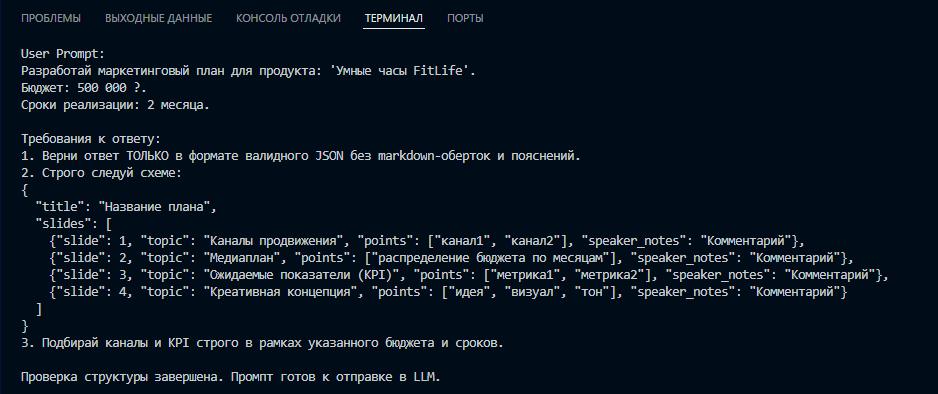
\includegraphics[width=16cm]{1.png}
		\caption{Результат тестирования класса PromptBuilder (вывод собранного промпта в консоль)}
	\end{figure}
	\newpage
	
	\section{Задание №2: Реализация программного взаимодействия с API}
	\subsection{Выбор API и параметры генерации}
	\noindent
	Использован Google AI Studio API с моделью \texttt{gemini-1.5-flash}. Модель оптимизирована для быстрой генерации структурированных данных и полностью бесплатна в рамках учебных квот.
	\begin{table}[H]
		\centering
		\begin{tabular}{|l|l|p{10cm}|}
			\hline
			\textbf{Параметр} & \textbf{Значение} & \textbf{Обоснование} \\ \hline
			temperature & 0.3 & Низкая температура для точного следования JSON-схеме и минимизации галлюцинаций в цифрах бюджета/KPI. \\ \hline
			top\_p & 0.9 & Обеспечивает достаточное разнообразие формулировок при сохранении строгости структуры. \\ \hline
		\end{tabular}
	\end{table}
	\noindent
	API-ключ хранится в секретах Google Colab (переменная \texttt{GOOGLE\_API\_KEY}), доступ через \texttt{userdata.get()}.
	
	\subsection{Реализация основного конвейера}
	\noindent
	Скрипт выполняет следующие шаги:
	\begin{enumerate}
		\item Создание экземпляра \texttt{MarketingPlanPromptBuilder} с переданными аргументами.
		\item Отправка запроса через Google Gemini с механизмом повторных попыток (Retry Logic) при сетевых ошибках.
		\item Автоматическая очистка ответа: поиск первого \texttt{\{} и последнего \texttt{\}}, удаление markdown-оберток.
		\item Валидация JSON через \texttt{json.loads()}. При ошибке формата генерируется запрос на самокоррекцию.
		\item Сохранение итоговых данных в \texttt{plan\_\{product\}.json} и форматированный \texttt{.txt} файл.
	\end{enumerate}
	
	\subsection{Листинг функций взаимодействия с API}
	\lstinputlisting{3.nonutf.txt}
	\newpage
	
	\subsection{Пример выполнения и структуры JSON-ответа}
	\begin{figure}[H]
		\centering
		
\includegraphics[width=16cm]{2.png}
		\caption{Результат выполнения программы (лог генерации и валидации)}
	\end{figure}
	\begin{figure}[H]
		\centering
		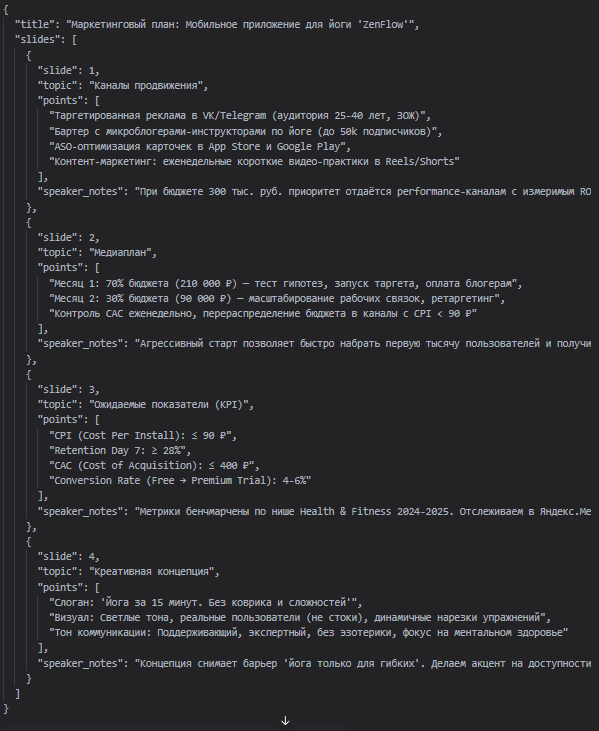
\includegraphics[width=16cm]{3.png}
		\caption{Фрагмент сгенерированного JSON-файла (структура слайдов)}
	\end{figure}
	\begin{figure}[H]
		\centering
		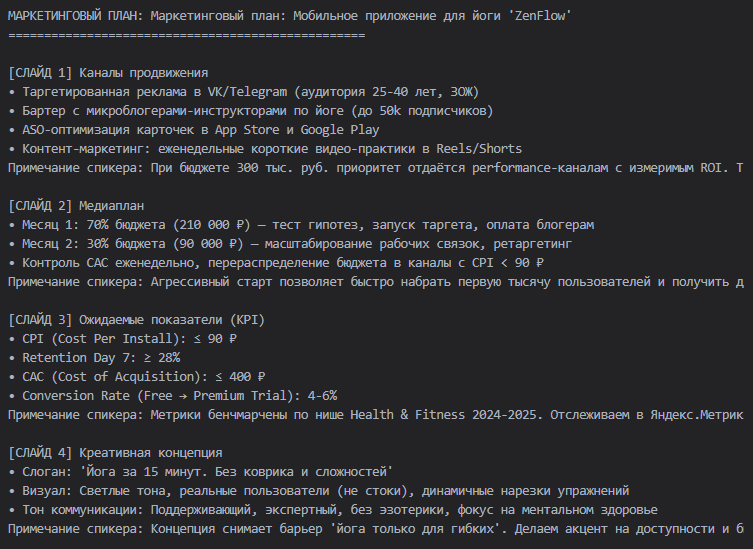
\includegraphics[width=16cm]{4.png}
		\caption{Отформатированный текстовый отчет для менеджера}
	\end{figure}
	\newpage
	
	\section{Задание №3: Тестирование, оценка качества и универсальности}
	\subsection{Тестовые сценарии}
	\noindent
	Программа запущена на трёх различных наборах входных данных:
	\begin{enumerate}
		\item Продукт «Мобильное приложение для йоги», Бюджет 300 000 ₽, Сроки 2 месяца
		\item Продукт «SaaS-платформа для HR», Бюджет 1 500 000 ₽, Сроки 3 месяца
		\item Продукт «Линейка органической косметики», Бюджет 500 000 ₽, Сроки 1 месяц
	\end{enumerate}
	
	\noindent
	\textbf{Пример «сырого» ответа модели до очистки:}
	\begin{verbatim}
		Вот структурированный маркетинговый план в формате JSON:
		```json
		{
			"title": "Маркетинговый план: Мобильное приложение для йоги",
			"slides": [...]
		}
	\end{verbatim}
	\newpage
	\subsection{Результаты тестирования}
	\begin{table}[H]
	\centering
	\begin{tabular}{|l|p{4cm}|p{3cm}|c|p{2.5cm}|p{3cm}|}
		\hline
		\textbf{Тест} & \textbf{Продукт} & \textbf{Бюджет} & \textbf{JSON валиден} & \textbf{Слайдов} & \textbf{KPI указаны} \ \hline
		1 & Приложение для йоги & 300 000 ₽ & Да & 4 & ROI, CAC, Retention \ \hline
		2 & SaaS для HR & 1 500 000 ₽ & Да & 4 & MRR, Churn, LTV \ \hline
		3 & Органическая косметика & 500 000 ₽ & Да & 4 & CTR, Conversion, ROMI \ \hline
	\end{tabular}
	\end{table}
	\subsection{Анализ ошибок и их исправление}
	\begin{table}[H]
	\centering
	\begin{tabular}{|l|p{5cm}|p{4.5cm}|p{4cm}|}
		\hline
		\textbf{№} & \textbf{Проблема} & \textbf{Корректировка} & \textbf{Результат} \ \hline
		1 & Модель добавляла markdown-обертку \texttt{```json} и приветствие & Реализован парсер с поиском первого \texttt{{} и последнего \texttt{}}, а также отсечением markdown & Извлечение JSON стало 100% стабильным \ \hline
		2 & В первом тесте KPI были слишком общими («увеличить продажи») & Усилен промпт: требование указывать конкретные метрики (CAC, LTV, ROMI, Retention) & Показатели стали измеримыми и профессиональными \ \hline
		3 & При малом бюджете модель предлагала неадекватные каналы (ТВ, наружка) & Добавлено условие в системный промпт: «Подбирай каналы строго в рамках указанного бюджета» & Медиаплан стал реалистичным и таргетированным \ \hline
	\end{tabular}
	\end{table}
	\noindent
	\textbf{Вывод по тестированию:} Инструмент успешно генерирует структурированные маркетинговые планы для продуктов разных ниш и бюджетов. Программа универсальна: изменение входных параметров не требует правки кода, а встроенная валидация гарантирует машиночитаемый результат.
	\newpage
	\section*{Заключение}
	\noindent
	\textbf{Оценка эффективности автоматизации:} Разработанный генератор маркетинговых планов сокращает время подготовки базовой структуры презентации с 2-3 часов ручного исследования и верстки до 30-50 секунд. Экономия времени составляет 180-360 раз при сохранении высокого уровня логической связности и профессиональной терминологии.
	\noindent
	\textbf{Выявленные ограничения:}
	\begin{itemize}
	\item Лимиты токенов: для очень детальных медиапланов может потребоваться постобработка или разбиение генерации по слайдам.
	\item Скорость API: в часы пиковой нагрузки Google AI Studio может отвечать с задержкой 5-10 сек.
	\item Актуальность цифр: модель генерирует прогнозные KPI на основе паттернов, требуется ручная валидация менеджером под реалии рынка.
	\end{itemize}
	\noindent
	\textbf{Наиболее эффективные техники промпт-инжиниринга:}
	\begin{itemize}
	\item Strict JSON Schema: жесткое описание структуры в промпте исключает вариативность ключей.
	\item Parameter Injection: динамическая подстановка бюджета и сроков позволяет модели адаптивно подбирать каналы.
	\item Self-Correction Loop: цикл валидации и повторного запроса при ошибке парсинга обеспечивает отказоустойчивость пайплайна.
	\item Separation of Concerns: класс \texttt{PromptBuilder} изолирует логику сборки запросов от сетевого взаимодействия.
	\end{itemize}
	\section*{Приложения}
	\noindent
	\textbf{Приложение А. Тестовые данные}
	\lstinputlisting[language=]{5.nonutf.txt}
	\noindent
	\textbf{Приложение Б. Ссылки} \
	Google Colab Notebook: \url{https://colab.research.google.com/drive/1DBsVTZJWpNhkiyBdpk7Hmhvl8ADKK0wW?usp=sharing} \
\end{document}